%------------------------------------------------------------------------------
% CV in Latex
% Author : Charles Rambo
% Based off of: https://github.com/sb2nov/resume and Jake's Resume on Overleaf
% Most recently updated version may be found at https://github.com/fizixmastr 
% License : MIT
%------------------------------------------------------------------------------

\documentclass[A4,11pt]{article}
%\documentclass[letterpaper,11pt]{article} %For use in US
\usepackage{latexsym}
\usepackage[empty]{fullpage}
\usepackage{titlesec}
\usepackage{marvosym}
\usepackage[usenames,dvipsnames]{color}
\usepackage{verbatim}
\usepackage{enumitem}
\usepackage[hidelinks]{hyperref}
\usepackage[english]{babel}
\usepackage{tabularx}
\usepackage{tikz}
\input{glyphtounicode}

\begin{comment}
I am by no means a professional when it comes to the CV's/resumes, I have
received various trainings on how to write a CV and resume from my high 
school, as well as the Austin College and University of Eastern Finland's
career counseling departments. As I intend to share my CV as a template, I 
feel that it is my responsibility to provide explanations of my work.
\end{comment}


%-----FONT OPTIONS-------------------------------------------------------------
\begin{comment}
The font of the document will impact not just how readable it is, but how it is
perceived. In the "The Craft of Scientific Writing" by Michael Alley, shares a
common fonts for publication as well as their use. I have chosen to use
Palatino for its legibility, some others are given below. There is far too much
about typography to discus here. Note: serif fonts have short projecting
strokes, sans-serif fonts are sans (without) these strokes.
\end{comment}


% serif
 \usepackage{palatino}
% \usepackage{times} %This is the default as well
% \usepackage{charter}

% sans-serif
% \usepackage{helvet}
% \usepackage[sfdefault]{noto-sans}
% \usepackage[default]{sourcesanspro}

%-----PAGE SETUP---------------------------------------------------------------

% Adjust margins
\addtolength{\oddsidemargin}{-1cm}
\addtolength{\evensidemargin}{-1cm}
\addtolength{\textwidth}{2cm}
\addtolength{\topmargin}{-1cm}
\addtolength{\textheight}{2cm}

% Margins for US Letter size
%\addtolength{\oddsidemargin}{-0.5in}
%\addtolength{\evensidemargin}{-0.5in}
%\addtolength{\textwidth}{1in}
%\addtolength{\topmargin}{-.5in}
%\addtolength{\textheight}{1.0in}

\urlstyle{same}

\raggedbottom
\raggedright
\setlength{\tabcolsep}{0cm}

% Sections formatting
\titleformat{\section}{
  \vspace{-4pt}\scshape\raggedright\large
}{}{0em}{}[\color{black}\titlerule \vspace{-5pt}]

% Ensure that .pdf is machine readable/ATS parsable
\pdfgentounicode=1

%-----CUSTOM COMMANDS FOR FORMATTING SECTIONS----------------------------------
\newcommand{\CVItem}[1]{
  \item\small{
    {#1 \vspace{-2pt}}
  }
}

\newcommand{\CVSubheading}[4]{
  \vspace{-2pt}\item
    \begin{tabular*}{0.97\textwidth}[t]{l@{\extracolsep{\fill}}r}
      \textbf{#1} & #2 \\
      \small#3 & \small #4 \\
    \end{tabular*}\vspace{-7pt}
}

\newcommand{\CVSubSubheading}[2]{
    \item
    \begin{tabular*}{0.97\textwidth}{l@{\extracolsep{\fill}}r}
      \text{\small#1} & \text{\small #2} \\
    \end{tabular*}\vspace{-7pt}
}

\newcommand{\CVSubItem}[1]{\CVItem{#1}\vspace{-4pt}}

\renewcommand\labelitemii{$\vcenter{\hbox{\tiny$\bullet$}}$}

\newcommand{\CVSubHeadingListStart}{\begin{itemize}[leftmargin=0.5cm, label={}]}
% \newcommand{\resumeSubHeadingListStart}{\begin{itemize}[leftmargin=0.15in, label={}]} % Uncomment for US
\newcommand{\CVSubHeadingListEnd}{\end{itemize}}
\newcommand{\CVItemListStart}{\begin{itemize}}
\newcommand{\CVItemListEnd}{\end{itemize}\vspace{-5pt}}

%------------------------------------------------------------------------------
% CV STARTS HERE  %
%------------------------------------------------------------------------------
\begin{document}

%-----HEADING------------------------------------------------------------------
\begin{comment}
In Europe it is common to include a picture of ones self in the CV. Select
which heading appropriate for the document you are creating.
\end{comment}

\begin{minipage}[c]{0.05\textwidth}
\-\
\end{minipage}
\begin{minipage}[c]{0.2\textwidth}
\begin{tikzpicture}
    \clip (0,-.7) circle (1.75cm);
    \node at (0,-.7) {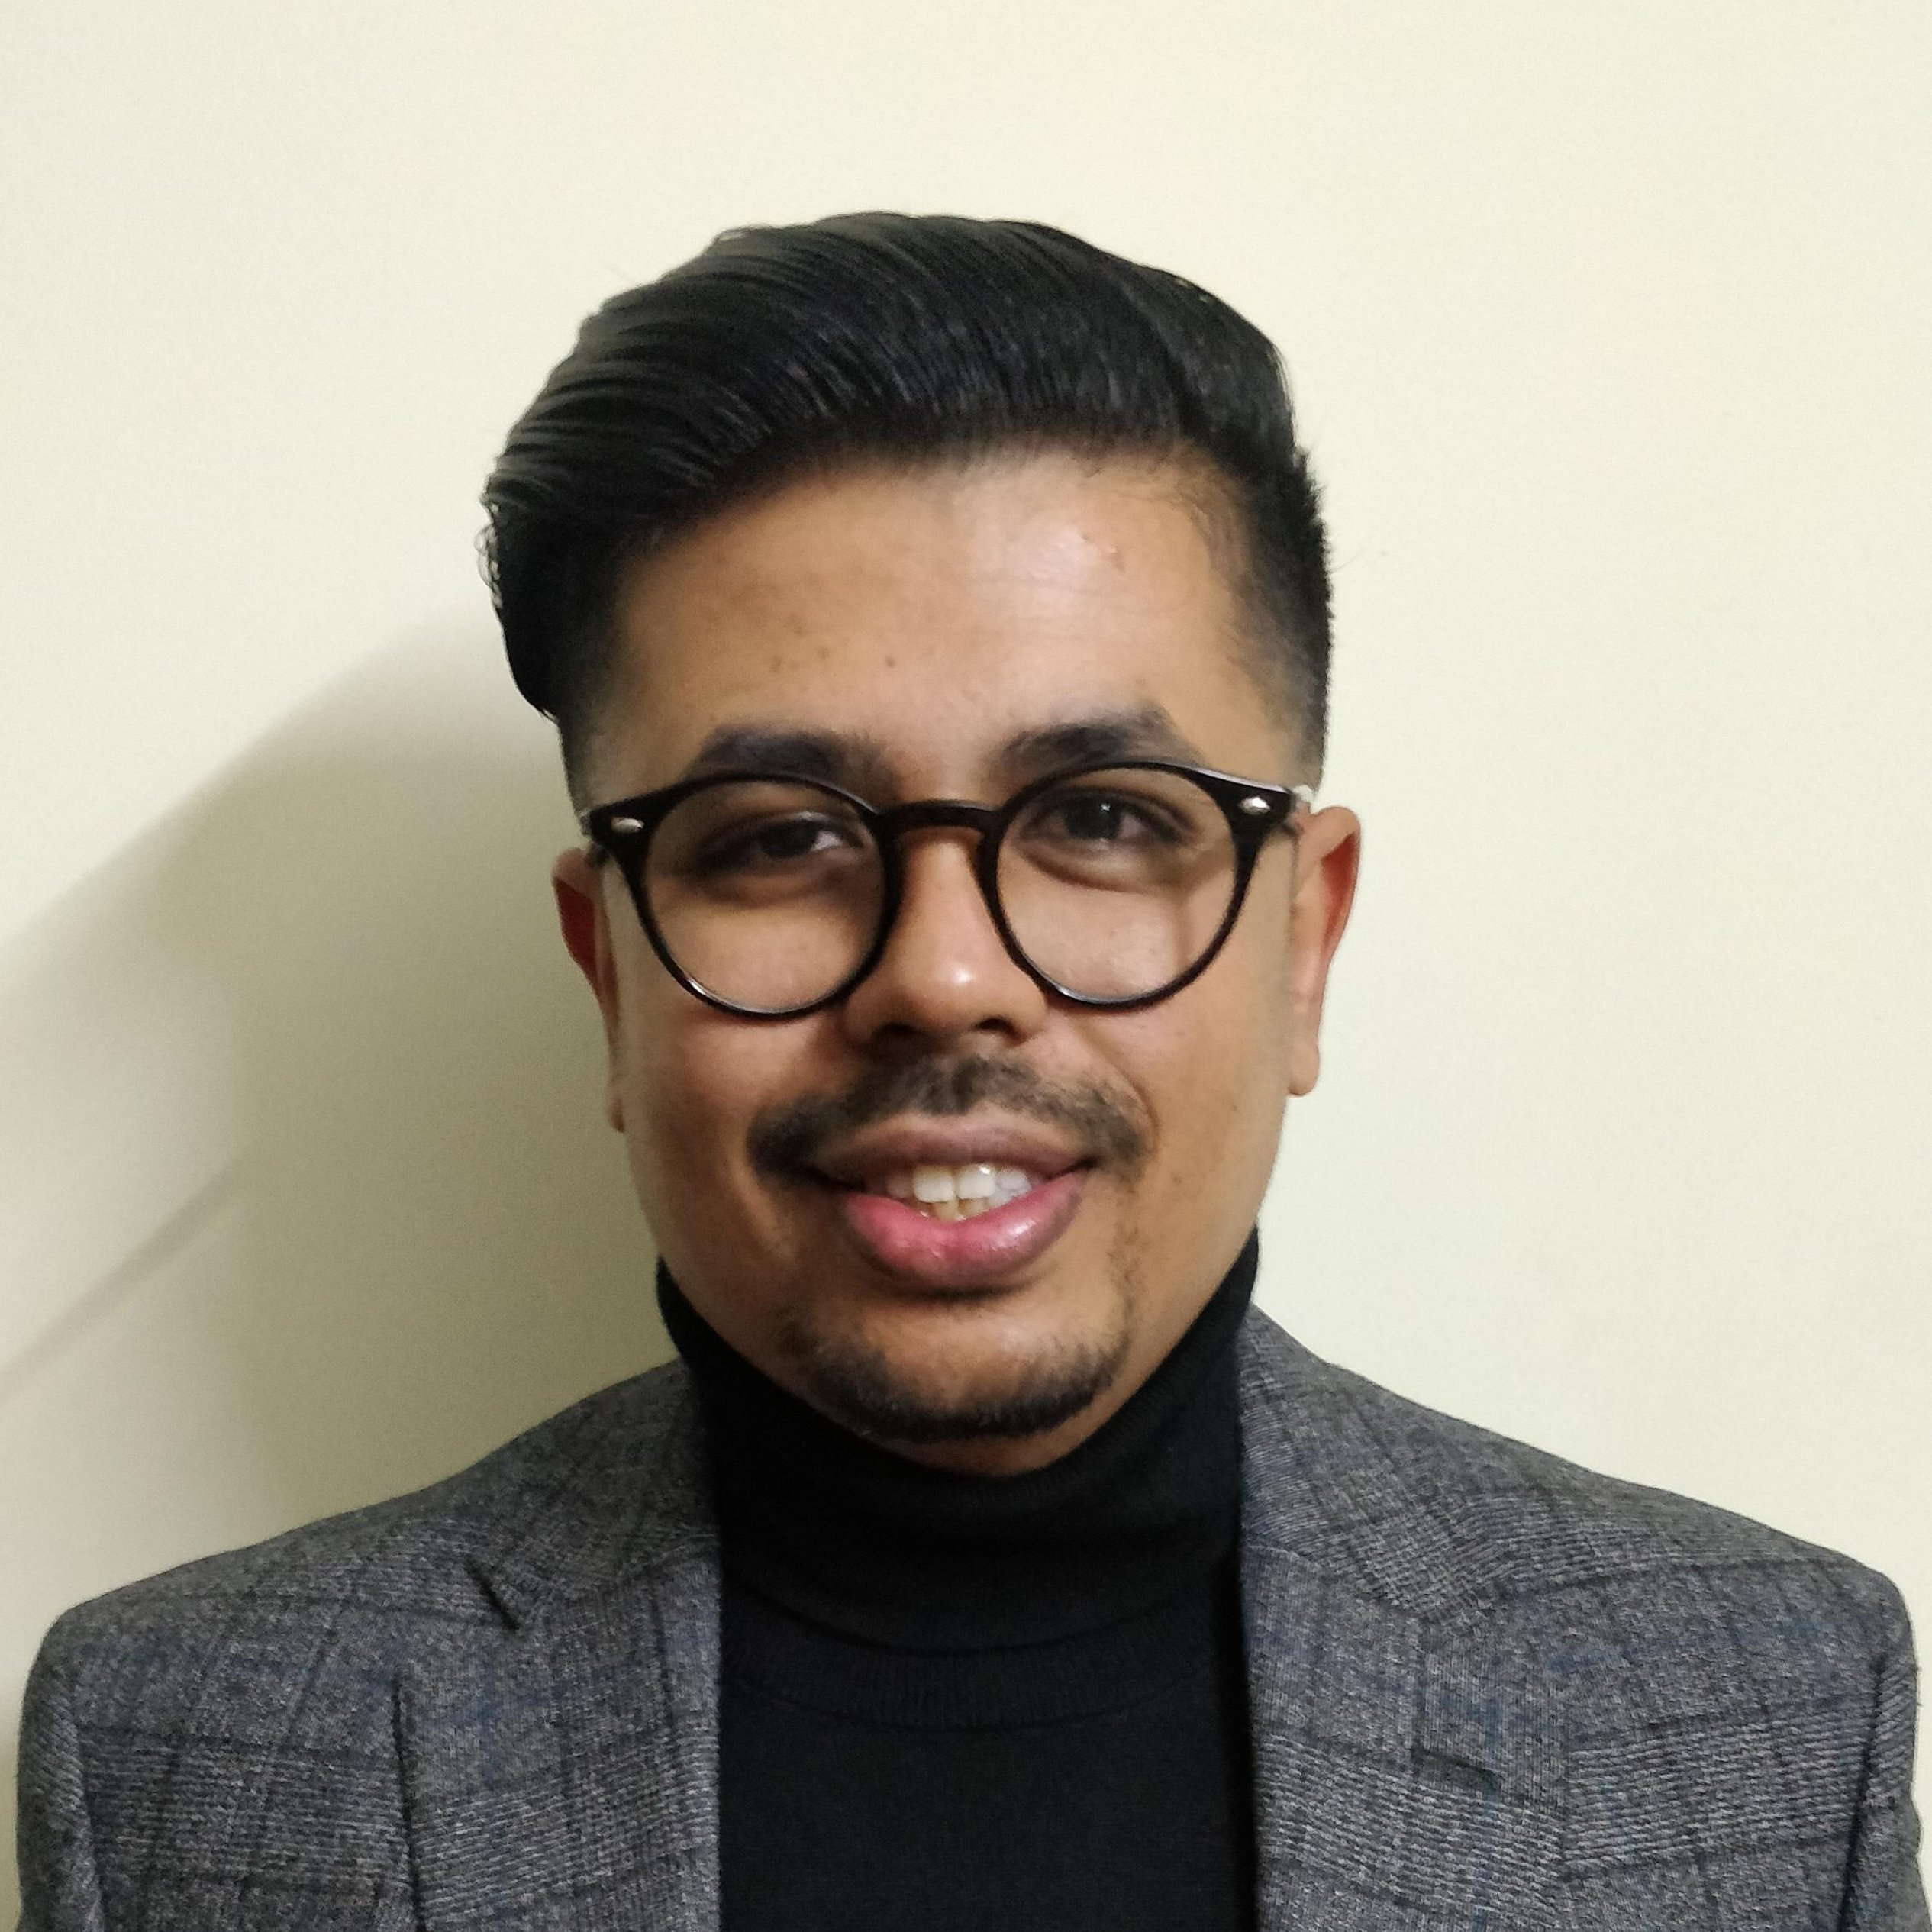
\includegraphics[width = 4cm]{photo}};
    % if necessary the picture may be moved by changing the at (coordinates)
    % width defines the 'zoom' of the picture
\end{tikzpicture}
\hfill\vline\hfill
\end{minipage}
\begin{minipage}[c]{0.4\textwidth}
    \textbf{\Large \scshape{\underline{Swapneel Amit Pathak}}} \\ \vspace{1pt}
    % \scshape sets small capital letters, remove if desired
    \href{mailto:swapneelap@gmail.com}{swapneelap@gmail.com}\\
    \small{+91-9879943726} \\
    % Be sure to use a professional *personal* email address
    % \href{https://www.linkedin.com/in/charles-rambo/}{\underline{linkedin.com/in/charles-rambo}} \\
    % you should adjust you linked in profile name to be professional and recognizable
    % \href{https://github.com/fiziuastr}{\underline{github.com/fizixmastr}}
\end{minipage}

% Without picture
%\begin{center}
%    \textbf{\Huge \scshape Charles Rambo} \\ \vspace{1pt} %\scshape sets small capital letters, remove if desired
%    \small +1 123-456-7890 $|$ 
%    \href{mailto:you@provider.com}{\underline{you@provider.com}} $|$\\
%    % Be sure to use a professional *personal* email address
%    \href{https://linkedin.com/in/your-name-here}{\underline{linkedin.com/in/charles-rambo}} $|$
%    % you should adjust you linked in profile name to be professional and recognizable
%    \href{https://github.com/fizixmastr}{\underline{github.com/fizixmastr}}
%\end{center}



\begin{comment}
This CV was written for specifically for positions I was applying for in
academia, and then modified to be a template.

A standard CV is about two pages long where as a resume in the US is one page.
sections can be added and removed here with this in mind. In my experience, 
education, and applicable work experience and skills are the most import things
to include on a resume. For a CV the Europass CV suggests the categories: Work
Experience, Education and Training, Language Skills, Digital Skills,
Communication and Interpersonal Skills, Conferences and Seminars, Creative Works
Driver's License, Hobbies and Interests, Honors and Awards, Management and
Leadership Skills, Networks and Memberships, Organizational Skills, Projects,
Publications, Recommendations, Social and Political Activities, Volunteering.

Your goal is to convey a who, what , when, where, why for every item you share. 
The who is obviously you, but I believe the rest should be done in that order.
For example below. An employer cares most about the degree held and typically 
less about the institution or where it is located (This is still good 
information though). Whatever order you choose be consistent throughout.
\end{comment}

%-----EDUCATION----------------------------------------------------------------
\section{Education}
  \CVSubHeadingListStart
%    \CVSubheading % Example
%      {Degree Achieved}{Years of Study}
%      {Institution of Study}{Where it is located}
    \CVSubheading
      {{Ph.D. $|$ \emph{\small{Physics}}}}{Aug 2017 -- Mar 2021}
      {University of Strasbourg}{Strasbourg, France}
    \CVSubheading
      {{Integrated Master of Science $|$ \emph{\small{Physics, Major: condensed
              matter physics}}}}{Jul 2009 -- May 2014}
      {Indian Institute of Technology Roorkee}{Roorkee, India}
  \CVSubHeadingListEnd

%-----WORK EXPERIENCE----------------------------------------------------------
\begin{comment}
try to briefly explain what you did and why it is relevant to the position you
are seeking
\end{comment}

\section{Work Experience}
  \CVSubHeadingListStart
%    \CVSubheading %Example
%      {What you did}{When you worked there}
%      {Who you worked for}{Where they are located}
%      \CVItemListStart
%        \CVItem{Why it is important to this employer}
%      \CVItemListEnd
    \CVSubheading
      {Visiting Scientist}{Oct 2021 -- present}
      {Scientific Support Unit for Computational Science, MPSD, CFEL}{Hamburg, Germany}
      \CVItemListStart
        \CVItem{Machine-learning models to cluster simulation data,
          extracting micromagnetic material parameters, and 3D reconstruction of
          magnetization field from experimental data}
        \CVItem{Magnetic skyrmion dynamics using vortex laser pulses}
        \CVItem{Accelerating micromagnetic simulation Python package using NVIDIA
          CUDA kernels}
      \CVItemListEnd
    \CVSubheading
      {Postdoctoral researcher}{Apr 2022 -- Jan 2023}
      {University of Southampton, Computational Modelling Group}{Southampton, UK}
      \CVItemListStart
        \CVItem{Developing and maintaining Ubermag (micromagnetic simulations in Python)}
        \CVItem{Unsupervised machine-learning algorithms to cluster micromagnetic simulation data}
      \CVItemListEnd
    \CVSubheading
    {Ph.D. Candidate (IdEx Fellow)}{Aug 2017 -- Mar 2021}
      {CNRS, IPCMS, University of Strasbourg}{Strasbourg, France}
      \CVItemListStart
        \CVItem{Numerical implementation of DMI in micromagnetism}
        \CVItem{Study of magnetic skyrmions in FeGe nanospheres}
        \CVItem{Skyrmion confinement in non-centrosymmetric ferromagnets}
      \CVItemListEnd
    \CVSubheading
    {Research Associate}{Jul 2015 -- Jul 2017}
     {Tata Institute of Fundamental Research (TIFR)}{Hyderabad, India}
      \CVItemListStart
        \CVItem{Study of magnetization dynamics in FM, AFM, and Insulator multi-layers with STT}
        \CVItem{Set up of Molecular Beam Epitaxy facility}
        \CVItem{FPGA based automation and differential pumping for Ultra High
          Vacuum (UHV)}
      \CVItemListEnd
    \CVSubheading
    {Research Assistant}{Apr 2015 -- Jun 2015}
     {Tata Institute of Fundamental Research (TIFR)}{Hyderabad, India}
      \CVItemListStart
        \CVItem{Simulation of magnetic multi-layers with OOMMF}
      \CVItemListEnd
    \CVSubheading
    {Research Assistant}{Jul 2014 -- Dec 2014}
     {Indian Institute of Science (IISc)}{Bangalore, India}
      \CVItemListStart
        \CVItem{Characterization of Au nanowires and graphene based gas sensors}
        \CVItem{Study of change in resistance noise of sensors due to physisorption of different gases}
      \CVItemListEnd
    \CVSubheading
    {Graduate Research Assistant}{May 2013 -- May 2014}
      {Indian Institute of Technology Roorkee}{Roorkee, India}
      \CVItemListStart
        \CVItem{Calculation of photonic band gaps using Finite Difference Time Domain (FDTD)}
      \CVItemListEnd
  \CVSubHeadingListEnd

% %-----PROJECTS AND RESEARCH----------------------------------------------------
% \begin{comment}
% Ideally the title of the work should speak for what it is. However if you feel
% like you should explain more about why the project is applicable to this job,
% use item list as is shown in the work experience section.
% \end{comment}

% \section{Projects and Research}
%   \CVSubHeadingListStart
% %    \CVSubheading
% %      {Title of Work}{When it was done}
% %      {Institution you worked with}{unused}
%     \CVSubheading
%       {{Surface Plasmon Propagation in the Kretschmann-Raether Configuration} $|$ \emph{\small{Python}}}{Fall 2020}
%       {University of Eastern Finland}{}
%     \CVSubheading
%       {{Simulation of Vector Beams Through High Numerical Aperture Lens} $|$ \emph{\small{Python}}}{Fall 2020}
%       {University of Eastern Finland}{}
%     \CVSubheading
%       {Characterization of the Flame-S Spectrometer for Spectral Imaging Research}{Spring 2020}
%       {University of Eastern Finland}{}
%     \CVSubheading
%       {{Free Form Lens Systems for 3D Printing} $|$ \emph{\small{MATLAB, OpTaliX}}}{Spring 2019}
%       {University of Eastern Finland}{}
%     \CVSubheading
%       {Procedures for Plating and Wet-Etching in III-V Semiconductor Devices}{Summer 2019}
%       {Finisar Corp.}{}
%     \CVSubheading
%       {Photo-Filter Characterization for Photometric Identification of Be Stars}{Fall 2017}
%       {Austin College}{}
%     \CVSubheading
%       {Improved Calibrating Equations for Volumetric Soil Moisture Measurement}{Spring 2017}
%       {Austin College}{}
%     \CVSubheading
%       {{Product Design, and Manufacturing Using 3D Printing} $|$ \emph{\small{Autodesk 123D}}}{Fall 2016}
%       {Austin College}{}
%   \CVSubHeadingListEnd

%-----CONFERENCES AND PRESENTATIONS--------------------------------------------
\begin{comment}
Again the title should have already been enough, but if it is necessary to add
descriptions maintain the consistency from prior sections
\end{comment}

\section{Conferences and Presentations}
  \CVSubHeadingListStart
%    \CVSubheading % Example
%      {Work Presented}{When}
%      {Occasion}{}
    \CVSubheading
    {Oral presentation at Conference on Magnetism and Magnetic Materials}{Nov 2022}
    {}{USA (Hybrid)}
    \CVSubheading
    {Workshop on Ubermag at SOL-SKYMAG 2022}{Jun 2022}
    {}{Spain}
    \CVSubheading
    {Oral Presentation at INTERMAG 2020}{May 2020}
    {}{Virtual}
    \CVSubheading
    {Oral Presentation at DPG Spring Meeting 2019}{Apr 2019}
    {}{Germany}
  \CVSubHeadingListEnd

%-----HONORS AND AWARDS--------------------------------------------------------
\section{Honors and Awards}
  \CVSubHeadingListStart
%    \CVSubheading %Example
%      {What}{When}
%      {Short Description}{}
    \CVSubheading
    {IdEx Fellow (Initiative for Excellence)}{Oct 2017 -- Mar 2021}
      {University of Strasbourg}{Strasbourg, France}
    \CVSubheading
    {INSPIRE Scholarship}{Jul 2009 -- May 2014}
      {Ministry of Science and Technology}{Roorkee, India}
  \CVSubHeadingListEnd

%-----TEACHING EXPERIENCE------------------------------------------------------
\begin{comment}
Section is here as it applied to my application for positions in academia. 
Remember to tailor the resume for to the position.
\end{comment}

\section{Teaching Experience}
  \CVSubHeadingListStart
%    \CVSubheading
%      {What}{When}
%      {School}{Where}
    \CVSubheading
      {Co-Supervised three M.Sc. thesis}{Jul 2022 -- Sep 2022}
      {Imperial College, London}{London, UK}
    \CVSubheading
      {Teaching under-privileged girls using flipped classroom
      technique}{Jan 2016 -- Jan 2017}
      {Tata Institute of Fundamental Research}{Hyderabad, India}
  \CVSubHeadingListEnd

%-----COMMUNITY INVOLVEMENT----------------------------------------------------
\section{Publications}
  \CVSubHeadingListStart
%    \CVSubheading %Example
%      {What you did}{When you worked there}
%      {Who you worked for}{Where they are located}
    \CVSubheading
      {}{}
      {S. J. R. Holt; M. Lang; J. C. Loudon; T. J. Hicken; D. Cortés-Ortuño;
        \textbf{S. A. Pathak}; M. Beg; H. Fangohr,\\
        Towards virtual micromagnetic experiments: mag2exp, \textit{in
        preparation for submission} 2022,\\ draft available
        \href{https://s.gwdg.de/8QRRcD}{\color{blue} \underline{here}}}{}
    \CVSubheading
      {}{}
      {\textbf{S. A. Pathak}; R. Hertel, Three-Dimensional Chiral Magnetization Structures in FeGe
        Nanospheres,\\ \textit{Physical Review B} 2021, 103, 104414}{}
    \CVSubheading
      {}{}
      {\textbf{S. A. Pathak}; R. Hertel, Geometrically Constrained Skyrmions,
        \textit{Magnetochemistry} 2021, 7(2), 26}{}
  \CVSubHeadingListEnd

%-----SKILLS-------------------------------------------------------------------
\begin{comment}
This section is compressed from the various skills sections that Euro CV
recommends.
\end{comment}

\section{Skills}
\begin{itemize}
  \item Micromagnetic and atomistic simulation studies of magnetic materials
  \item Epitaxial growth and characterisation of magnetic thin films in
    ultra-high vacuum
  \item Implementation of machine learning algorithms in study of magnetic
    materials
  \item Software engineering: Version control, unit tests, CI/CD
  \item Maintenance and setup of High Performance Computation (HPC) clusters
  \item Programming skill in Python, C/C++, Rust, Bash, and MATLAB
\end{itemize}
% -----REFERENCES--------------------------------------------------------------
\section{Reference}
\CVSubHeadingListStart
\CVSubheading
{Prof. Hans Fangohr}{MPSD, CFEL}
{\href{mailto:hans.fangohr@mpsd.mpg.de}{hans.fangohr@mpsd.mpg.de}}{Hamburg, Germany}
\CVSubheading
{Dr. habil. Riccardo Hertel}{IPCMS, CNRS}
{\href{mailto:hertel@ipcms.unistra.fr}{hertel@ipcms.unistra.fr}}{Strasbourg, France}
\CVSubHeadingListEnd
\end{document}